\documentclass[paper=letter, fontsize=11pt]{scrartcl} % Letter paper and 11pt font size

\usepackage{amstext, amsmath, amssymb, graphicx}
\usepackage[T1]{fontenc} % Use 8-bit encoding that has 256 glyphs
\usepackage[english]{babel} % English language/hyphenation
\usepackage{amsmath,amsfonts,amsthm} % Math packages

\usepackage{fancyhdr} % Custom headers and footers
\pagestyle{fancyplain} % Makes all pages in the document conform to the custom headers and footers
\fancyhead{} % No page header
\fancyfoot[L]{} % Empty left footer
\fancyfoot[C]{} % Empty center footer
\fancyfoot[R]{\thepage} % Page numbering for right footer
\renewcommand{\headrulewidth}{0pt} % Remove header underlines
\renewcommand{\footrulewidth}{0pt} % Remove footer underlines
\setlength{\headheight}{13.6pt} % Customize the height of the header
\setlength\parindent{0pt} % Remove all indentation from paragraps.


%----------------------------------------------------------------------------------------
%	TITLE SECTION
%----------------------------------------------------------------------------------------

\newcommand{\horrule}[1]{\rule{\linewidth}{#1}} % Create horizontal rule command with 1 argument of height

\title{	
\normalfont \normalsize 
\textsc{San Francisco State University} \\ [25pt]
\horrule{0.5pt} \\[0.4cm] % Thin top horizontal rule
\huge MATH 490 Assignment 3 \\ % The assignment title
\horrule{2pt} \\[0.5cm] % Thick bottom horizontal rule
}

\author{Omar Sandoval}

\date{\normalsize\today}

\begin{document}

\maketitle

%----------------------------------------------------------------------------------------
%	PROBLEM 2.18
%----------------------------------------------------------------------------------------
\textbf{2.18}	Table 2.13 shows data from the 2002 General Social Survey cross classifying
a person's perceived happiness with their family income. The table displays the observed
and expected cell counts and the standardized residuals for testing independence. \\

\textbf{a.}	Show how to obtain the estimated expected cell count of 35.8 for the first cell.
\\
To find the estimated expected cell count we can take (Sum of Not Too Happy)(Sum of Above
Average)/n = $\dfrac{(168)(290)}{1362}$ \\

\textbf{b.} For testing independence, $X^2 = 73.4$. Report the $df$ value and the P-value, 
and interpret. \\
We can find $df = (I-1)+(J-1) = (2)+(2) = 4$ \\
P-value is less than $0.0001$ so there is very strong evidence of an association. \\

\textbf{c.} Interpret the standardized residuals in the corner cells having counts 21 and 
83. \\
Corner Cell $\pi_{11}$: $\dfrac{n_{11} - \hat{\mu}_{11}}{\sqrt{\hat{\mu}(1-p_{1+})(1
-p_{+1})}} = \dfrac{(21)-(35.8)}{\sqrt{35.8(1-(290/1362))(1-(168/1362))}}$ //
$ = \dfrac{14.8}{4.97}= -2.97 $
\\
Corner Cell $\pi_{33}$: $\dfrac{n_{33} - \hat{\mu_{33}}}{\sqrt{\hat{\mu}(1-p_{3+})(1
-p_{+3})}} = -5.907$. \\

There is strong evidence that there are less people in those cells from the population
 than if the variables were independent of each other. In the first cell, the number is 
 2.97 standard errors smaller than the estimated expected.

\textbf{d.} Interpret the standardized residuals in the corner cells having counts 110 and
94. \\
There is strong evidence that there are more people in these cells than if the variables were independent.

\begin{center}
	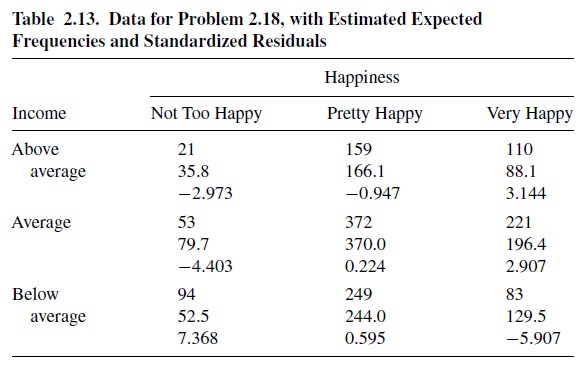
\includegraphics[scale=.55]{table213.png}
\end{center}
%----------------------------------------------------------------------------------------
%	PROBLEM 2.21
%----------------------------------------------------------------------------------------
\textbf{2.21} Each subject in a sample of 100 men and 100 women is asked to indicate which
of the following factors (one or more) are responsible for increases in teenage crime. A,
the increasing gap in income between the rich and poor; B, the increase in the percentage
of single-parent families; C, insufficient time spent by parents with their children. A 
cross classification of the responses by gender is \\

\begin{center}
	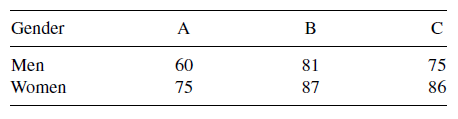
\includegraphics[scale=.75]{contTable221.png}
\end{center}

\textbf{a.} Is it valid to apply the chi-squared test of independence to this $2 \times 3$
table? Explain. \\
No it is not valid. The reason being because the columns are all dependent since the
subjects were able to select as many columns as they pleased. \\

\textbf{b.} Explain how this table actually provides information needed to cross-classify
gender with each of three variables. Construct the contingency table relating gender to
opinion about whether factor A is responsible for increases in teenage crime. \\

\begin{tabular}{lll}
Gender & Yes & No        \\
Men    & 60  & 100-60=40 \\
Women  & 75  & 100-75=25 \\
\end{tabular}
\\

%----------------------------------------------------------------------------------------
%	PROBLEM 2.22
%----------------------------------------------------------------------------------------
\textbf{2.22} Table 2.15 classifies a sample of psychiatric patients by their diagnosis
and by whether their treatment prescribed drugs. \\

\textbf{a.} Conduct a test of independence, and interpret the P-value. \\

$H_0$: $\pi_{ij} = \pi_i * \pi_j \forall i, j$. \\
$H_a$: $\pi_{ij} = \pi_i * \pi_j$ for some $i, j$. \\
Pearson Chi-Squared test: $X^2 = \sum \dfrac{(n_{ij} - \hat{\mu}_{ij})^2}{\hat{\mu}_{ij}}$
$ = 84.1888$ with degree of freedom 4.

This distribution has a mean of $df = 4$ and standard deviation of 84.1888 and a p-value that is close to 0. We can conclude that the diagnosis of the patients is associated to whether their treatment prescribed drugs or not. \\

\textbf{b.} Obtain standardized residuals, and interpret. \\

We can find standardized residuals with $\dfrac{n_{ij}-\hat{\mu}_{ij}}{\sqrt{\hat{\mu}_{ij}(1-p_i)(1-p_j)}}$.

\begin{tabular}{l}
$\hat{\mu}_{11} = \dfrac{(113)(182)}{276}=74.5145$ \\
$\hat{\mu}_{12} = \dfrac{(113)(94)}{276}=38.4855$  \\
$\hat{\mu}_{21} = \dfrac{(14)(182)}{276}=9.2319$   \\
$\hat{\mu}_{22} = \dfrac{(14)(94)}{276}=4.7681$    \\
$\hat{\mu}_{31} = \dfrac{(37)(182)}{276}=24.3986$  \\
$\hat{\mu}_{32} = \dfrac{(37)(94)}{276}=12.6014$   \\
$\hat{\mu}_{41} = \dfrac{(99)(182)}{276}=65.2826$  \\
$\hat{\mu}_{42} = \dfrac{(99)(94)}{276}=33.7174$   \\
$\hat{\mu}_{51} = \dfrac{(13)(182)}{276}=8.5725$   \\
$\hat{\mu}_{52} = \dfrac{(13)(94)}{276}=4.4275$   
\end{tabular}
\\

Residuals:
\begin{tabular}{|l|l|l|}
\hline
Diagnosis            & Drugs   & No Drugs \\ \hline
Schizophrenia        & 7.8742  & -7.8745  \\ \hline
Affective disorder   & 1.6022  & -1.6023  \\ \hline
Neurosis             & -2.3853 & 2.3852   \\ \hline
Personality disorder & -4.8416 & 4.8418   \\ \hline
Special symptoms     & -5.1393 & 5.1396   \\ \hline
\end{tabular}
\\

Each cell lacks similarity between $n_{ij}$ and $\hat{\mu}_{ij}$ that would be obvious
is the variables were actually truly independent. \\

\begin{center}
	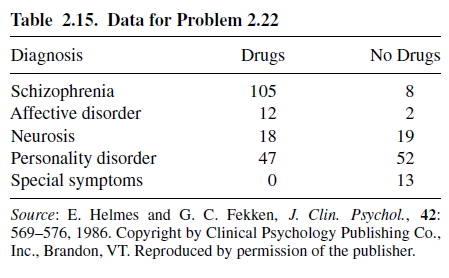
\includegraphics[scale=.75]{table215.png}
\end{center}

\textbf{c.} Partition chi-squared into three components to describe differences and
similarities among the diagnoses, by comparing (i) the first rows, (ii) the third and
fourth rows, (iii) the last row to the first and second rows combined and the third
and fourth rows combined. \\

(i)
We take X = Diagnosis, and Y = Treatment. X can either be Schizophrenia (1) and Affective
Disorder (2). \\
$H_0: \pi_{ij} = \pi_{i+}\pi_{+j}$ for all i = 1,2 and j = 1,2. \\
$H_a: \pi_{ij} = \pi_{i+}\pi_{+j}$ for some i and j. \\
$n = 127, I = 2, J = 2, \alpha = .05$ \\ 
$X^2 = \sum_{i=1}^{2}\sum_{j=1}^{2} \dfrac{(n_{ij}-\hat{\mu}_{ij})^2}{\hat{\mu}_{ij}}$ \\
We reject the null hypothesis when $X^2 > \chi_{1,0.05}^2 = 3.84$. \\
$X^2 = .3855$ with p-value $= .3450$. \\
We do not reject the null hypthesis at 0.05 level of significance. There is not enough evidence to conclude there is a relationship between Diagnosis and Treatment when partitioned between Schizophrenia and Affective Disorder. \\

(ii)
We take X = Diagnosis, and Y = Treatment. X can either be Neurosis (1) and Personality
Disorder (2). \\
$H_0: \pi_{ij} = \pi_{i+}\pi_{+j}$ for all i = 1,2 and j = 1,2. \\
$H_a: \pi_{ij} = \pi_{i+}\pi_{+j}$ for some i and j. \\
$n = 136, I = 2, J = 2, \alpha = .05$ \\ 
$X^2 = \sum_{i=1}^{2}\sum_{j=1}^{2} \dfrac{(n_{ij}-\hat{\mu}_{ij})^2}{\hat{\mu}_{ij}}$ \\
We reject the null hypothesis when $X^2 > \chi_{1,0.05}^2 = 3.84$. \\
$X^2 = .0149$ with p-value $= .9029$. \\
We do not reject the null hypothesis at 0.05 level of significance. There is not enough
evidence to conclude that there is a relationship between Neurosis and Peronality
Disorder. \\

(iii)
We take X = Diagnosis, and Y = Treatment. X can either be Schizophrenia/Affective
Disorder (1), Neurosis/Personality Disorder (2), or Special Diagnosis (3). \\
$H_0: \pi_{ij} = \pi_{i+}\pi_{+j}$ for all i = 1,2,3 and j = 1,2. \\
$H_a: \pi_{ij} = \pi_{i+}\pi_{+j}$ for some i and j. \\
$n = 276, I = 3, J = 2, \alpha = .05$ \\ 
$X^2 = \sum_{i=1}^{3}\sum_{j=1}^{2} \dfrac{(n_{ij}-\hat{\mu}_{ij})^2}{\hat{\mu}_{ij}}$ \\
We reject the null hypothesis when $X^2 > \chi_{2,0.05}^2 = 3.84$. \\
$X^2 = 83.8839$ with p-value $= .0001$. \\
We reject the null hypothesis at the 0.05 level of significance. There is sufficient
evidence for us to conclude that there is a strong relationship between Diagnosis and
Treatment when partitioned as Schizophrenia/Affective Disorder, Neurosis/Personality
Disorder or Special Symptoms. We can also note that Special Symptoms are never treated
with drugs while Neurosis, Personality Disorder are almost equally likely to be
treated with or without drugs. \\

%----------------------------------------------------------------------------------------
%	PROBLEM 2.30
%----------------------------------------------------------------------------------------
\textbf{2.30} Table 2.17 contains results of a study comparing radiation therapy with
surgery in treating cancer of the larynx. User Fisher's exact test to test $H_0: \theta =
1$ against $H_a: \theta > 1$. Interpret results. \\

\begin{center}
	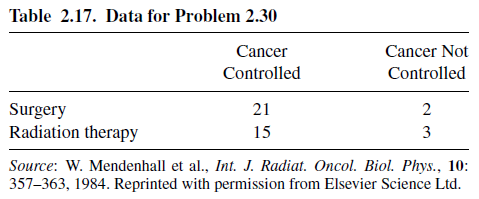
\includegraphics[scale=.75]{table217.png}
\end{center}

P-value is .6384. We fail to reject the null hypothesis and conclude the treatment of cancer
is independent of surgery and radiation therapy. \\

%----------------------------------------------------------------------------------------
%	PROBLEM 2.33
%----------------------------------------------------------------------------------------
\textbf{2.33} In murder trials in 20 Florida counties during 1976 and 1977, the death penalty was given in 19 out of 151 cases in which a white killed a white, in 0 out of 9 cases in 
which a white killed a black, in 11 out of 63 cases in which a black killed a white, and 
in 6 out of 103 cases in which a black killed a black. (M. Radelet, \textit{Am. Sociol. 
Rev.,} \textbf{46}: 918-927, 1981). \\

\textbf{a.} Exhibit the data as a three-way contingency table. \\

\begin{tabular}{|l|l|l|l|}
\hline
Defendant & Victim & Yes & No  \\ \hline
White     & White  & 19  & 132 \\ \hline
White     & Black  & 0   & 9   \\ \hline
Black     & White  & 11  & 52  \\ \hline
Black     & Black  & 6   & 97  \\ \hline
\end{tabular}
\\

\textbf{b.} Construct the partial tables needed to study the conditional association 
between defendant's race and the death penalty verdict. Find and interpret the sample
conditional odds ratios, adding 0.5 to each cell to reduce the impact of the 0 cell count.
\\

White Victim\\
\begin{tabular}{|l|l|l|}
\hline
Defendant & Yes & No  \\ \hline
White     & 19  & 132 \\ \hline
Black     & 11  & 52  \\ \hline
\end{tabular}
\\

Black Victim\\ 
\begin{tabular}{|l|l|l|}
\hline
Defendant & Yes & No \\ \hline
White     & 0   & 9  \\ \hline
Black     & 6   & 97 \\ \hline
\end{tabular}

Conditional Odds Ratio for when victim is white; $\dfrac{19.5 \times 52.5}{132.5 \times
11.5} = 0.6719$ \\
This odds ratio is less than 1, so we can conclude when the victim is white, a black defendant
is more likely to have a death penalty than a white defendant. \\

Conditional Odds Ratio for when victim is black: $\dfrac{0.5 \times 97.5}{9.5 \times 6.5}
= .7895$\\
This odds ratio is less than 1, so we can conclude when the victim is black, a black defendant
is more likely to have a death penalty than a white defendant.

In conclucsion, a black defendant is more likely to have a death penalty than a white
defendant regardless of a victim's race. \\

\textbf{c.} Compute and interpret the sample maginal odds ratio between defendant's race
and the death penalty verdict. Do these data exhibit Simpson's paradox? Explain. \\

\begin{tabular}{|l|l|l|}
\hline
Defendant's Race & Yes & No  \\ \hline
White            & 19  & 141 \\ \hline
Black            & 17  & 149 \\ \hline
\end{tabular}
\\
Odds ratio between defendant's race and the death penalty verdict; $\dfrac{19 \times 149}
{141 \times 17} = 1.1811$. \\
This odds ratio is greater than 1, so we can conclude that a white defendant is more likely
to have a death penalty compared to a black defendant without regard to a victim's race. \\
Simpson's paradox is valid in this case, since what we infered from the conditional and marginal odds ratios are contradictory. \\

%----------------------------------------------------------------------------------------
%	PROBLEM 2.38
%----------------------------------------------------------------------------------------
\textbf{2.38} For three-way contingency tables: \\

\textbf{a.} When any pair of variables is conditionally independent, explain why there is
homogeneous association. \\

When we have homogeneous association between X and Y, then we have
$\theta_{XY(1)} = \theta_{XY(2)}$ or $\theta_{XZ(1)} = \theta_{XZ(2)}$. The XY conditional
odds ratio equals 1 at each Z. Here, the odds are all equal at all levels of Z, and thus
there is homogeneous association. \\


\textbf{b.} When there is not homogeneous association, explain why no pair of variables can
be conditionally independent. \\

If there is no homogeneous association then no pair of variables can be associated homogeneously
 and therefore cannot be conditionally independent.\\

\end{document}
